\newpage
\section{Metodologia Experimental}

\subsection{Materiais}
O material utilizado foi:
\begin{itemize}
\item 1 potenciômetro $10k \Omega$;
\item 1 resistor $10k \Omega$;
\item 1 potenciômetro $1k \Omega$;
\item 2 resistores de 1 $k\Omega$;
\item 10 peças de peso (roscas);
\item 1 sensor \textit{strain gauge};
\item 1 ampop INA125;
\item fonte de alimentação ajustável;
\item multímetro;
\item software MATLAB.
\end{itemize}

Para execução do experimento, faz-se necessário executar os seguintes passos:

\begin{enumerate}
\item montar o circuito da figura \ref{f_sch}, substituindo RG por um potenciômetro de 1$k\Omega$;
\item Ajustar as fontes de tensão variável para +12V e -12V;
\item Ajustar RG para $V_{out} = 5V$ quando o sensor estiver com 10 peças;
\item Adicionar as peças, uma de cada vez, anotando os valores de tensão na saída;
\item Montar o gráfico massa x $V_{out}$;.
\end{enumerate}

\begin{figure}[H]
    \centering
    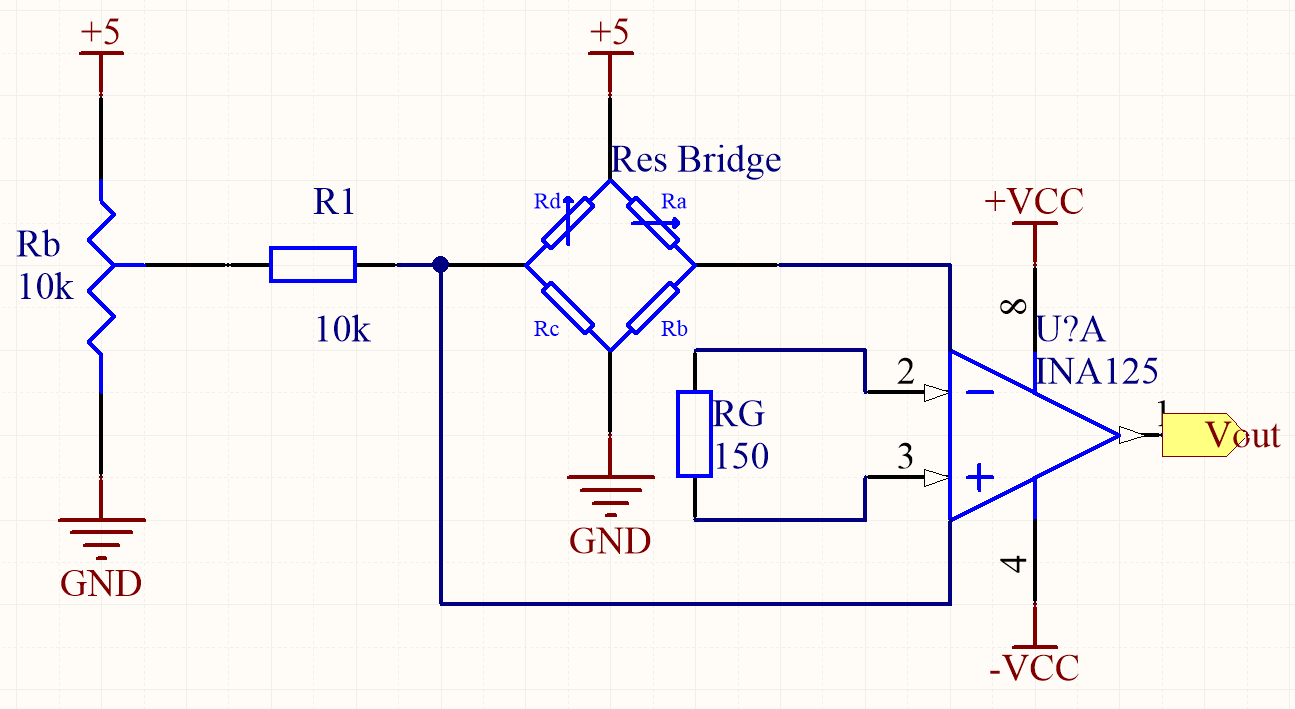
\includegraphics[scale=0.5]{img/sch.png}
    \caption{Circuito de acoplamento para o sensor \textit{strain gauge}.}
    \label{f_sch}
\end{figure}